\documentclass[a4paper]{article}

% Packages
\usepackage[14pt]{extsizes}
\usepackage[T2A]{fontenc}
\usepackage[russian]{babel}
\usepackage[left=20mm, top=15mm, right=15mm, bottom=20mm]{geometry}
\usepackage{graphicx} % For images
\usepackage{amsmath, amssymb} % For equations
\usepackage{booktabs} % For better tables
\usepackage{pgfplots} % For plotting graphs
\usepackage{xcolor} % For color support
\usepackage{caption} % For captioning tables and figures
\usepackage{float} % For precise float placement (images, tables)
\usepackage{array} % For better table management
\usepackage[hidelinks]{hyperref} % For table of contents to be clickable
\usepackage{bookmark}
\usepackage{multirow}
\usepackage{array}
\usepackage{cancel}
\usepackage{placeins}
\usepackage{enumitem}
\pgfplotsset{compat=1.17}

% Importing custom definitions (lstset, tikzset, etc.)
% % listing for programming code blocks
% listing for Python code blocks
\lstset{
	language=python,                 % Programming language
	basicstyle=\ttfamily\small,      % Adjust font size
	keywordstyle=\color{blue}\bfseries,  % Style for keywords
	stringstyle=\color{red},         % Style for strings
	commentstyle=\color{gray}\itshape, % Style for comments
	morecomment=[l][\color{magenta}]{\#}, % Special comment style for Python comments
	breaklines=true,                 % Line breaking in long lines
	numbers=left,                    % Line numbering on the left
	numberstyle=\tiny\color{gray},   % Style for line numbers
	frame=single,                    % Code frame
	showstringspaces=false,          % Don't show spaces in strings
	captionpos=b,                    % Caption position (b = bottom)
	tabsize=4,                       % Adjust tab spacing
	rulecolor=\color{black},         % Color of the frame
	emph={self},                     % Specific highlighting for keywords like 'self'
	emphstyle=\color{teal},          % Style for emphasized words (like 'self')
}

% \input{../common/tikzset.tex}

% -------------------------------

\begin{document}

% Title page
\input{../../common/title-old.tex}
\thispagestyle{empty}

\newpage
\pagestyle{plain}
\setcounter{page}{1}

% -------------------------------

% autogenerated table of contents
\linespread{0.9}
\tableofcontents
\linespread{1}

% -------------------------------

\newpage
\section*{Цель работы}
Изучение методов обработки и статистического анализа результатов измерений на примере
заданной числовой последовательности путем оценки числовых моментов и выявления свойств
последовательности на основе корреляционного анализа, а также аппроксимация закона
распределения заданной последовательности по двум числовым моментам случайной величины.


% -------------------------------

\section{Расчёт числовых моментов заданной ЧП}
В данной работе рассматривается случайная числовая последовательность (ЧП), для которой требуется рассчитать основные числовые моменты. Что значит \textit{случайная}? Значит состоит из случайных величин, то есть набора значений, полученных в результате наблюдений или экспериментов. Числовые моменты используются для описания характеристик распределения таких данных.

В этой работе для различных выборок случайной величины (10, 20, 50, 100, 200 и 300 значений) были рассчитаны следующие числовые моменты:
\begin{itemize}
	\item математическое ожидание;
	\item дисперсия;
	\item среднеквадратическое отклонение;
	\item коэффициент вариации;
	\item доверительные интервалы.
\end{itemize}

\subsection{Математическое ожидание}
\textbf{Математическое ожидание} — это среднее значение случайной величины, которое показывает её центр распределения. Это важный числовой момент, который описывает центр масс распределения данных, если простыми словами -- какая величина наиболее ``ожидаема`` в выборке.

Математическое ожидание для выборки из $n$ значений вычисляется по следующей формуле:
\[
	\mu = \frac{1}{n} \sum_{i=1}^{n} x_i
\]
где $n$ — количество элементов в выборке, $x_i$ — значение $i$-го элемента.


\subsection{Дисперсия}
\textbf{Дисперсия} показывает степень разброса значений относительно математического ожидания. Она позволяет оценить, насколько сильно данные отклоняются от среднего значения.

Дисперсия для выборки вычисляется по формуле:
\[
	\sigma^2 = \frac{1}{n - 1} \sum_{i=1}^{n} (x_i - \mu)^2
\]
где $\mu$ — математическое ожидание, $n$ — количество элементов выборки.

В этой работе дисперсия рассчитывается для каждой подвыборки, чтобы оценить, как изменяется разброс значений по мере увеличения объёма выборки.

\subsection{Среднеквадратическое отклонение}
\textbf{Среднеквадратическое отклонение (СКО)} — это квадратный корень из дисперсии. Оно показывает стандартную величину отклонения значений от их среднего. Обратите внимание, я сказал ``стандартную`` величины, потому что этот показатель также называется стандартным отклонением.

СКО вычисляется по формуле:
\[
	\sigma = \sqrt{\sigma^2}
\]
Вопрос, а зачем нужен СКО если дисперсия уже показывает вариабельность данных? Потому что он позволяет оценить отклонение значений от среднего \textit{в тех же} единицах измерения, что и исходные данные, что делает его более интуитивно понятным.

\subsection{Коэффициент вариации}
\textbf{Коэффициент вариации} представляет собой отношение стандартного отклонения к математическому ожиданию и выражается в процентах. Этот показатель используется для оценки относительного разброса данных и полезен при сравнении данных с разными средними значениями.

Формула коэффициента вариации:
\[
	CV = \frac{\sigma}{\mu} \times 100\%
\]

\subsection{Доверительные интервалы}
\textbf{Доверительный интервал} — это диапазон значений, в который с определённой вероятностью попадает истинное математическое ожидание. В данной работе использовались доверительные интервалы для уровней доверия 0.9, 0.95 и 0.99.

Формула для расчёта доверительного интервала:
\[
	CI = \mu \pm t_{\alpha/2} \cdot \frac{\sigma}{\sqrt{n}}
\]
где $t_{\alpha/2}$ — критическое значение $t$-распределения для заданного уровня доверия, $\sigma$ — стандартное отклонение, $n$ — объём выборки.

Чем больше объём выборки, тем уже доверительный интервал, что означает более точную оценку математического ожидания.

\subsection{Форма 1: Таблица числовых моментов для различных выборок}
В таблице ниже представлены числовые моменты для выборок из 10, 20, 50, 100, 200 и 300 значений. Для каждой подвыборки вычислены математическое ожидание, дисперсия, среднеквадратическое отклонение, коэффициент вариации и доверительные интервалы для различных уровней доверия, а также относительные отклонения рассчитанных значений от величин, полученных для выборки из 300 значений.

\begin{table}[h]
	\centering
	\resizebox{\textwidth}{!}{
		\begin{tabular}{|c|c|c|c|c|c|c|c|}
			\hline
			\multirow{2}{*}{\textbf{Характеристика}}   &      & \multicolumn{6}{c|}{\textbf{Количество случайных величин}}                                                                                        \\
			\cline{2-8}
			                                           &      & \textbf{10}                                                & \textbf{20} & \textbf{50} & \textbf{100} & \textbf{200} & \textbf{300}               \\
			\hline
			\multirow{2}{*}{\textbf{Мат. ожидание}}    & Знач & 147.476                                                    & 148.874     & 162.476     & 181.411      & 178.538      & \multirow{2}{*}{175.513}   \\
			\cline{2-7}
			                                           & $\%$ & -15.974                                                    & -15.178     & -7.428      & 3.360        & 1.723        &                            \\
			\hline
			\multirow{2}{*}{\textbf{Дов. инт. (0.9)}}  & Знач & \pm28.544                                                  & \pm26.761   & \pm23.416   & \pm19.893    & \pm14.512    & \multirow{2}{*}{\pm11.701} \\
			\cline{2-7}
			                                           & $\%$ & \pm143.937                                                 & \pm128.699  & \pm100.119  & \pm70.008    & \pm24.018    &                            \\
			\hline
			\multirow{2}{*}{\textbf{Дов. инт. (0.95)}} & Знач & \pm35.224                                                  & \pm32.392   & \pm28.068   & \pm23.773    & \pm17.316    & \multirow{2}{*}{\pm13.956} \\
			\cline{2-7}
			                                           & $\%$ & \pm152.392                                                 & \pm132.100  & \pm101.113  & \pm70.339    & \pm24.077    &                            \\
			\hline
			\multirow{2}{*}{\textbf{Дов. инт. (0.99)}} & Знач & \pm 50.604                                                 & \pm44.277   & \pm37.431   & \pm31.467    & \pm22.838    & \multirow{2}{*}{\pm18.385} \\
			\cline{2-7}
			                                           & $\%$ & \pm175.250                                                 & \pm140.836  & \pm103.599  & \pm71.159    & \pm24.225    &                            \\
			\hline
			\multirow{2}{*}{\textbf{Дисперсия}}        & Знач & 2424.613                                                   & 4790.369    & 9753.900    & 14354.424    & 15422.509    & \multirow{2}{*}{15088.212} \\
			\cline{2-7}
			                                           & $\%$ & -83.930                                                    & -68.251     & -35.354     & -4.863       & 2.216        &                            \\
			\hline
			\multirow{2}{*}{\textbf{Ср. кв. о.}}       & Знач & 49.240                                                     & 69.212      & 98.762      & 119.810      & 124.187      & \multirow{2}{*}{122.834}   \\
			\cline{2-7}
			                                           & $\%$ & -59.913                                                    & -43.654     & -19.597     & -2.462       & 1.102        &                            \\
			\hline
			\multirow{2}{*}{\textbf{Коэф. вариации}}   & Знач & 33.389\%                                                   & 46.491\%    & 60.786\%    & 66.043\%     & 69.558\%     & \multirow{2}{*}{69.986}    \\
			\cline{2-7}
			                                           & $\%$ & -52.292                                                    & -33.571     & -13.146     & -5.633       & -0.611       &                            \\
			\hline
		\end{tabular}}
	\caption{Числовые моменты для различных выборок ЧП}
\end{table}

\subsection{Выводы}
Проведя рассчёт числовых моментов заданной числовой последовательности можно сделать однозначный вывод о том, что при росте количества случайных величин (т.е. объёма выборки) -- отклонения рассчитанных значений относительно самой большой выборки в 300 элементов \textbf{уменьшаются} (по модулю), как уменьшается погрешность полученных величин и точность эксперимента соответственно.


% -------------------------------

\newpage
\section{Графический анализ последовательности}
\subsection{График числовой последовательности}
График заданной числовой последовательности имеет следующий вид:

\begin{figure}[H]
	\centering
	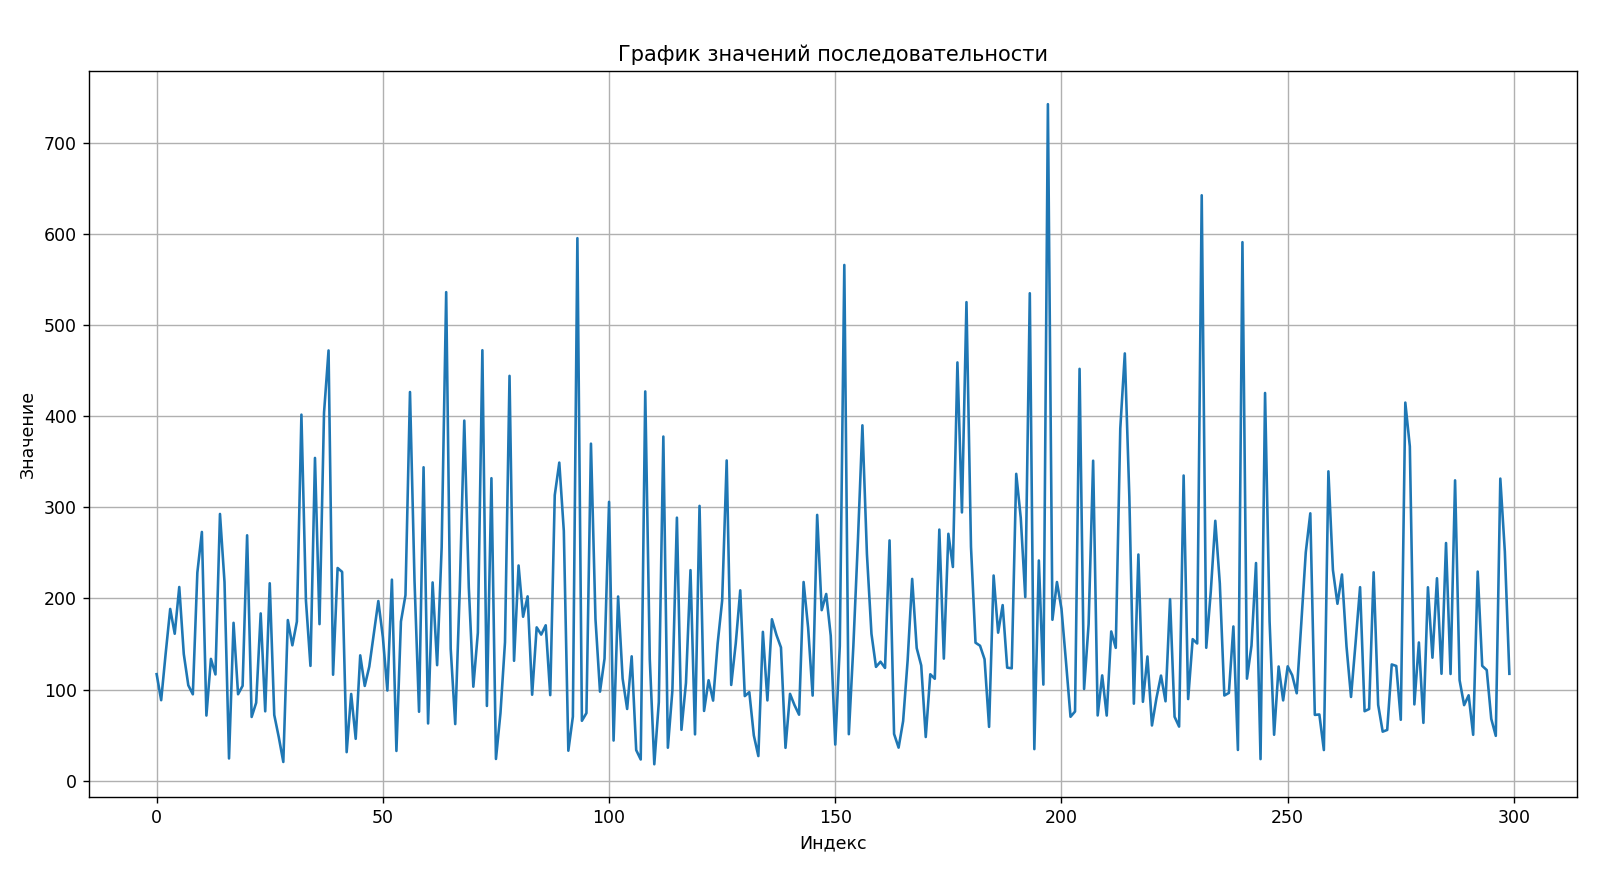
\includegraphics[width=1\textwidth]{../data/sequence.png}
	\caption{График числовой последовательности}
\end{figure}

\subsection{Анализ числовой последовательности}

Построив график числовой последовательности (Рис. 1), можно провести её анализ и определить характер распределения значений:

\begin{itemize}
	\item \textbf{Тренд (возрастающая/убывающая последовательность)}: График не демонстрирует явной тенденции роста или падения. Значения колеблются в случайном порядке, не показывая направленного изменения в какую-либо сторону. Следовательно, последовательность \textbf{не является ни возрастающей, ни убывающей}.

	\item \textbf{Периодичность}: На графике отсутствуют чёткие повторяющиеся паттерны. Это позволяет заключить, что последовательность \textbf{не является периодичной}.

	\item \textbf{Случайный характер}: Видимые колебания значений на графике происходят без какой-либо закономерности. Это указывает на \textbf{случайный характер} последовательности.
\end{itemize}

\subsection{Вывод}

Таким образом, по результатам анализа можно сделать вывод, что исследуемая числовая последовательность является \textbf{хаотичной} и не демонстрирует признаков \textbf{ни периодичности}, \textbf{ни направленного} изменения.


% -------------------------------

\section{Автокорреляционный анализ}
Автокорреляция — это метод оценки зависимости значений последовательности от её предыдущих значений. Она показывает, насколько текущее значение данных связано с предыдущими, и позволяет определить наличие закономерностей или зависимости в данных.

\textbf{Автокорреляционный анализ} — это исследование временной зависимости данных, направленное на выявление структур или закономерностей. Важно понимать, что высокий коэффициент автокорреляции для определённого сдвига указывает на наличие зависимости между текущими и предыдущими значениями. Если коэффициенты автокорреляции невелики, это свидетельствует о случайной природе последовательности.

\subsection{Выполнение автокорреляционного анализа}

В таблице ниже представлены коэффициенты автокорреляции для различных сдвигов (от 1 до 10) как для исходной последовательности, так и для сгенерированной числовой последовательности.

\begin{table}[H]
	\centering
	\resizebox{\textwidth}{!}{
		\begin{tabular}{|c|c|c|c|c|c|c|c|c|c|c|}
			\hline
			\textbf{Сдвиг ЧП}                     & \textbf{1} & \textbf{2} & \textbf{3} & \textbf{4} & \textbf{5} & \textbf{6} & \textbf{7} & \textbf{8} & \textbf{9} & \textbf{10} \\
			\hline
			\textbf{К-т АК} для зад. \textbf{ЧП}  & -0.0206    & -0.0099    & 0.0579     & 0.0680     & -0.0160    & -0.0047    & 0.0170     & -0.0307    & -0.0334    & 0.0260      \\
			\hline
			\textbf{К-т АК} для сген. \textbf{ЧП} & -0.0464    & 0.0167     & 0.0242     & -0.0350    & 0.0909     & -0.0560    & -0.0495    & -0.0452    & -0.0632    & -0.0089     \\
			\hline
			\textbf{\% откл.}                     & 125.243    & -268.687   & -58.204    & -151.471   & -668.125   & 1091.49    & -391.176   & 47.231     & 89.222     & -65.769     \\
			\hline
		\end{tabular}
	}
	\caption{Коэф. автокорреляции для заданной и сгенерированной ЧП}
\end{table}

\subsection{Результаты автокорреляционного анализа}

Для оценки случайности последовательности использовалось пороговое значение коэффициента автокорреляции — 0.2. Если автокорреляция на сдвиге превышает это значение, последовательность можно считать неслучайной. Но как видно из талицы и графика, ни одно из значений коэффициентов корелляции для исходной последовательности не превышает даже 0,1 -- исходя из этого можно сделать вывод, что числовая последовательность является случайной.

\begin{figure}[H]
	\centering
	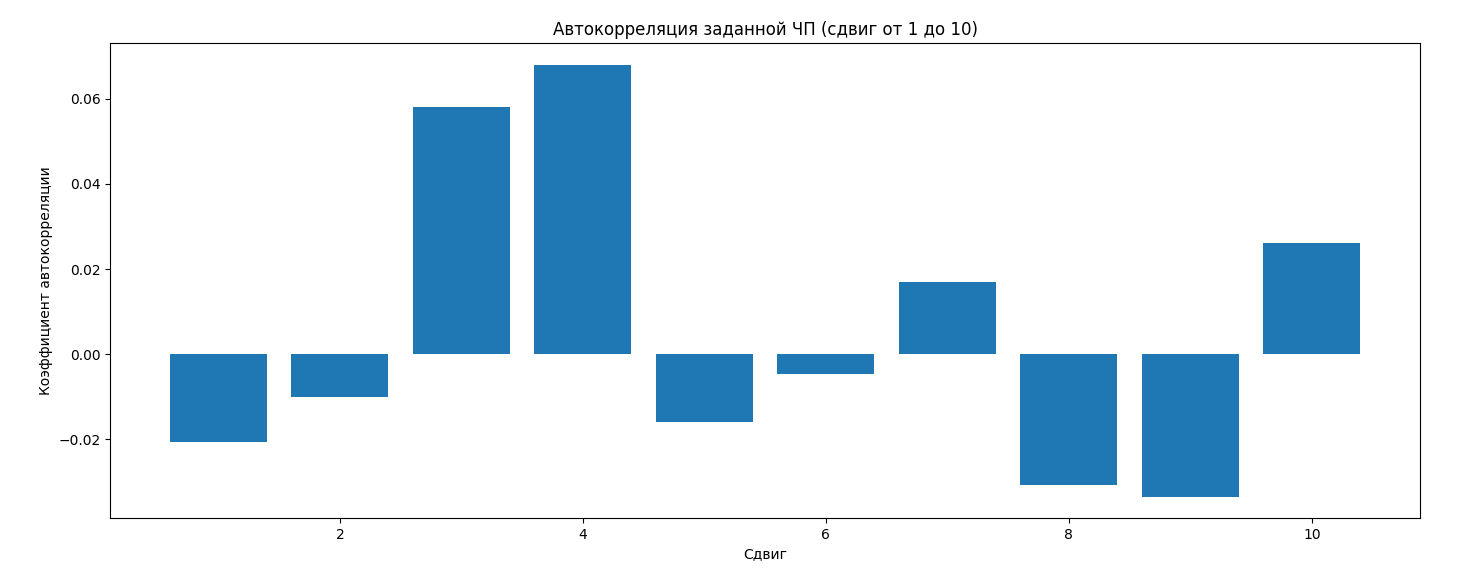
\includegraphics[width=1\textwidth]{../data/auto_corellation-1.png}
	\caption{Автокорреляционный анализ для заданной ЧП}
\end{figure}


\subsection{Анализ сгенерированной последовательности}

\begin{figure}[H]
	\centering
	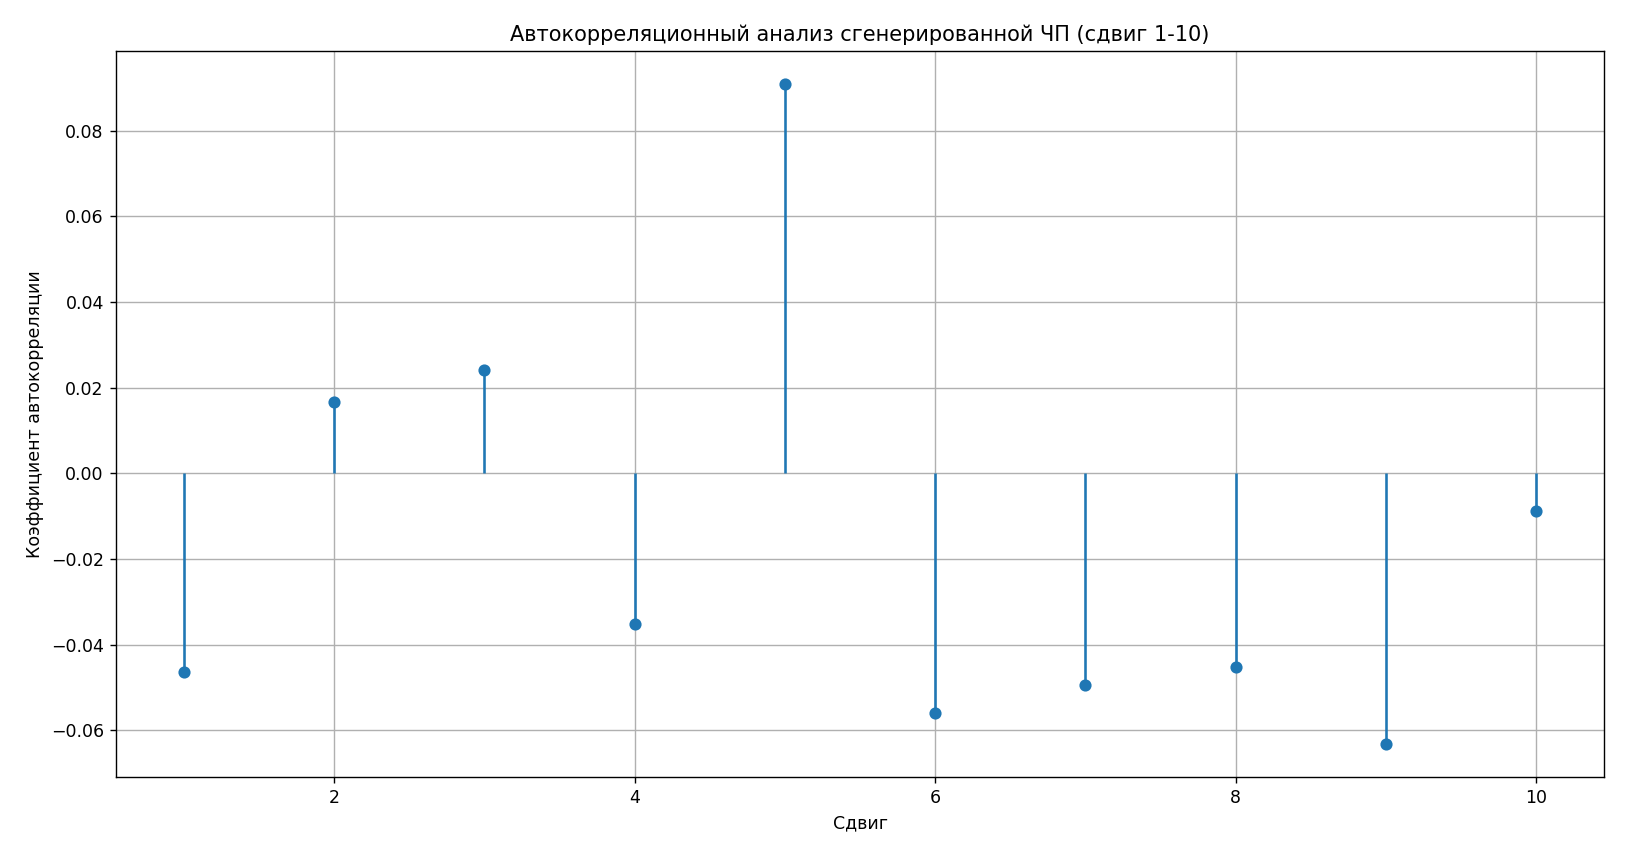
\includegraphics[width=1\textwidth]{../data/auto_corellation-2.png}
	\caption{Автокорреляционный анализ для сгенерированной числовой последовательности}
\end{figure}

Аналогичный анализ был проведён для сгенерированной числовой последовательности. Как показано на графике и в таблице, все коэффициенты автокорреляции для сгенерированной последовательности также не превышают порога 0.1, что позволяет заключить, что сгенерированная последовательность является случайной.

\subsection{Выводы}

На основании автокорреляционного анализа можно сделать следующие выводы:
\begin{itemize}
	\item Заданная числовая последовательность не имеет значимых зависимостей между значениями на различных сдвигах. Все коэффициенты автокорреляции для сдвигов от 1 до 10 не превышают порога 0.1, что позволяет считать последовательность \textbf{случайной}.
	\item Сгенерированная числовая последовательность также демонстрирует случайный характер, так как коэффициенты автокорреляции не превышают значения 0.1.
\end{itemize}


% -------------------------------

\section{Гистограмма распределения частот заданной ЧП}
\subsection{График гистограммы распределения частот}

\FloatBarrier
\begin{figure}[h]
	\centering
	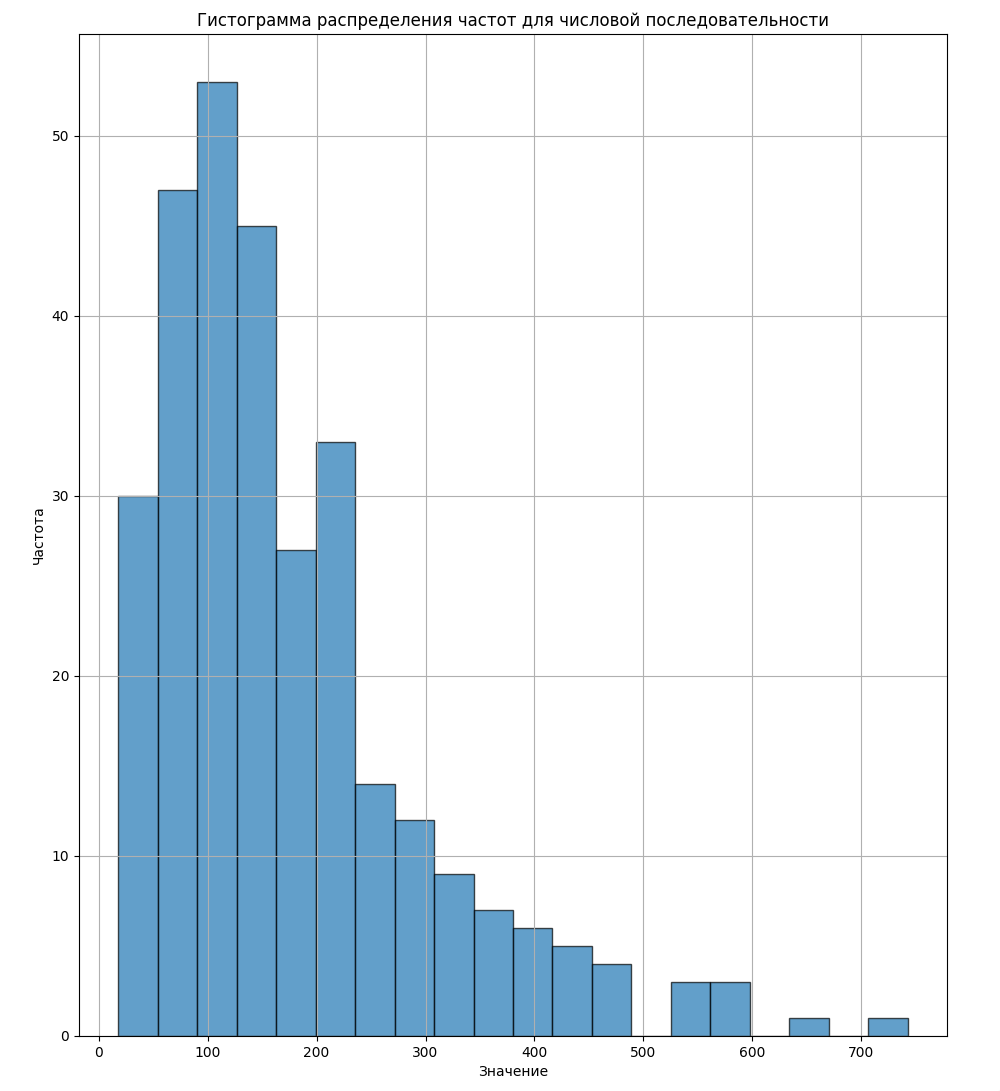
\includegraphics[width=0.7\textwidth]{../data/histogram.png}
	\caption{Гистограмма распределения частот заданной ЧП}
\end{figure}
\FloatBarrier

\subsection{Анализ и вывод}

Построенная гистограмма (рис. 1) представляет распределение частот для числовой последовательности. На графике можно заметить, что большинство значений сосредоточены в области с малыми числами, а частота встречаемости значений резко снижается по мере увеличения значений.

Такой характер распределения данных указывает на \textbf{экспоненциальное распределение}. Это видно из резкого спада частоты по мере увеличения величины, что является характерной чертой экспоненциального распределения.


% -------------------------------

\section{Анализ вида аппроксимирующего закона распределения заданной ЧП}
% На основе значения коэффициента вариации \(CV\), рассчитанного для различных подвыборок, было выбрано распределение, аппроксимирующее заданную случайную последовательность:

\begin{itemize}
	\item Для подвыборок с количеством случайных величин 10, 20, 50, 100, 200 и 300 значения коэффициента вариации составляют \(33.389\%\), \(46.491\%\), \(60.786\%\), \(66.043\%\), \(69.558\%\), и \(69.986\%\) соответственно.
	\item Так как все значения коэффициента вариации находятся в диапазоне \(0 < CV < 100\%\), было выбрано \textbf{нормированное распределение Эрланга k-го порядка} для аппроксимации закона распределения. Это распределение подходит для данных с коэффициентом вариации ниже \(100\%\), где распределение менее дисперсно по сравнению с экспоненциальным.
\end{itemize}

Функция плотности вероятности для распределения Эрланга k-го порядка имеет вид:

\[
	f(x; k, \lambda) = \frac{\lambda^k x^{k-1} e^{-\lambda x}}{(k-1)!}
\]
где \(k\) — порядок распределения, \(\lambda\) — параметр, обратный среднему значению.

Например, для различных $k$ и $\lambda$ распределения Эрланга может принимать следующий вид (Рис. 5). Чтобы понять какой характерен нашей ЧП, надо произвести расчёт параметров для распределения Эрланга.

\FloatBarrier
\begin{figure}[h]
	\centering
	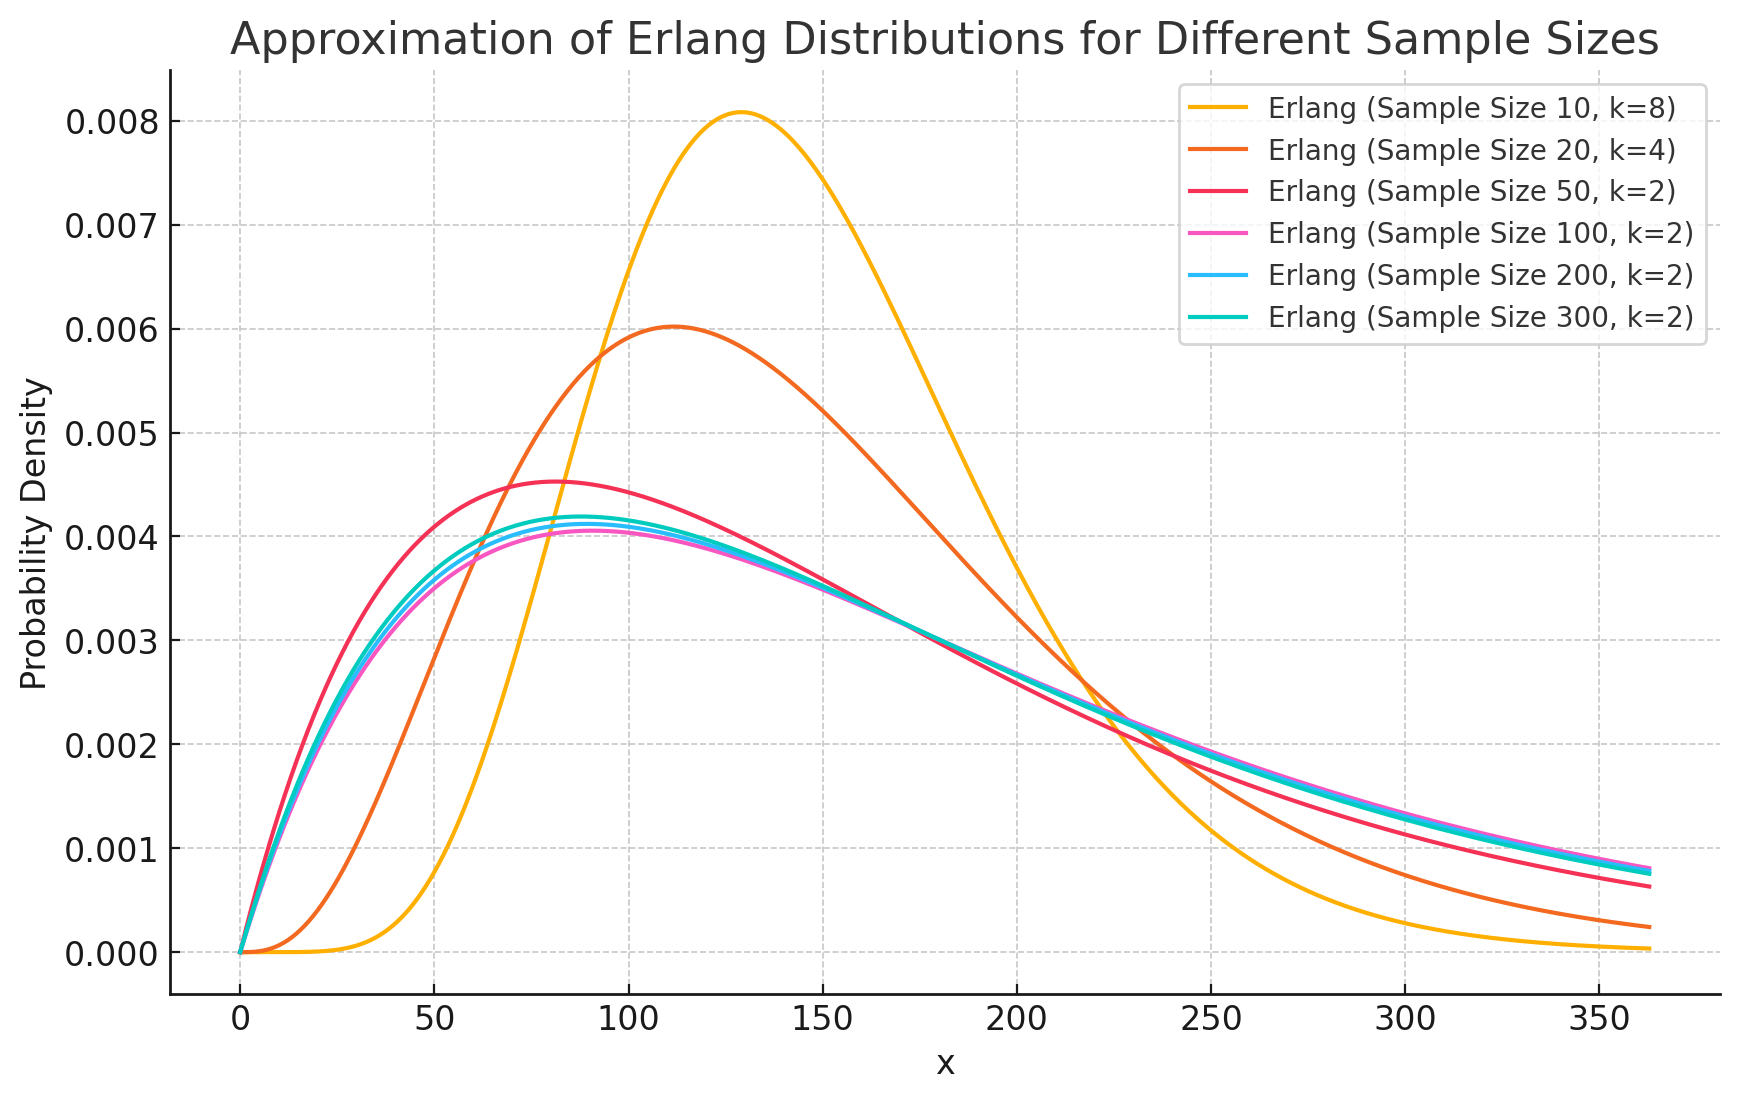
\includegraphics[width=1\textwidth]{../data/histogram_example.png}
	\caption{Распределение Эрланга для различных параметров}
\end{figure}
\FloatBarrier

\subsection{Расчёт параметров распределения Эрланга}

\begin{enumerate}
	\item Для последовательности из 300 элементов у нас есть следующие данные:
	      \[
		      \mu = 175.5133 \quad \text{(математическое ожидание)}
	      \]
	      \[
		      \sigma^2 = 15088.212 \quad \text{(дисперсия)}
	      \]

	\item Теперь мы можем рассчитать порядок \(k\) распределения Эрланга по формуле:
	      \[
		      k = \frac{\mu^2}{\sigma^2}
	      \]
	\item Подставляем значения:
	      \[
		      k = \frac{175.5133^2}{15088.212} = \frac{30714.96}{15088.212} \approx 2.036
	      \]
	\item Округляем до ближайшего целого числа:
	      \[
		      k \approx 2
	      \]

	\item Далее рассчитываем параметр масштаба \( \lambda \) по формуле:
	      \[
		      \lambda = \frac{k}{\mu}
	      \]
	\item Подставляем значения:
	      \[
		      \lambda = \frac{2}{175.5133} \approx 0.0114
	      \]

	\item Таким образом, для последовательности из 300 элементов параметры распределения Эрланга следующие:
	      \[
		      k = 2, \quad \lambda = 0.0114
	      \]

\end{enumerate}


\FloatBarrier
\begin{figure}[h]
	\centering
	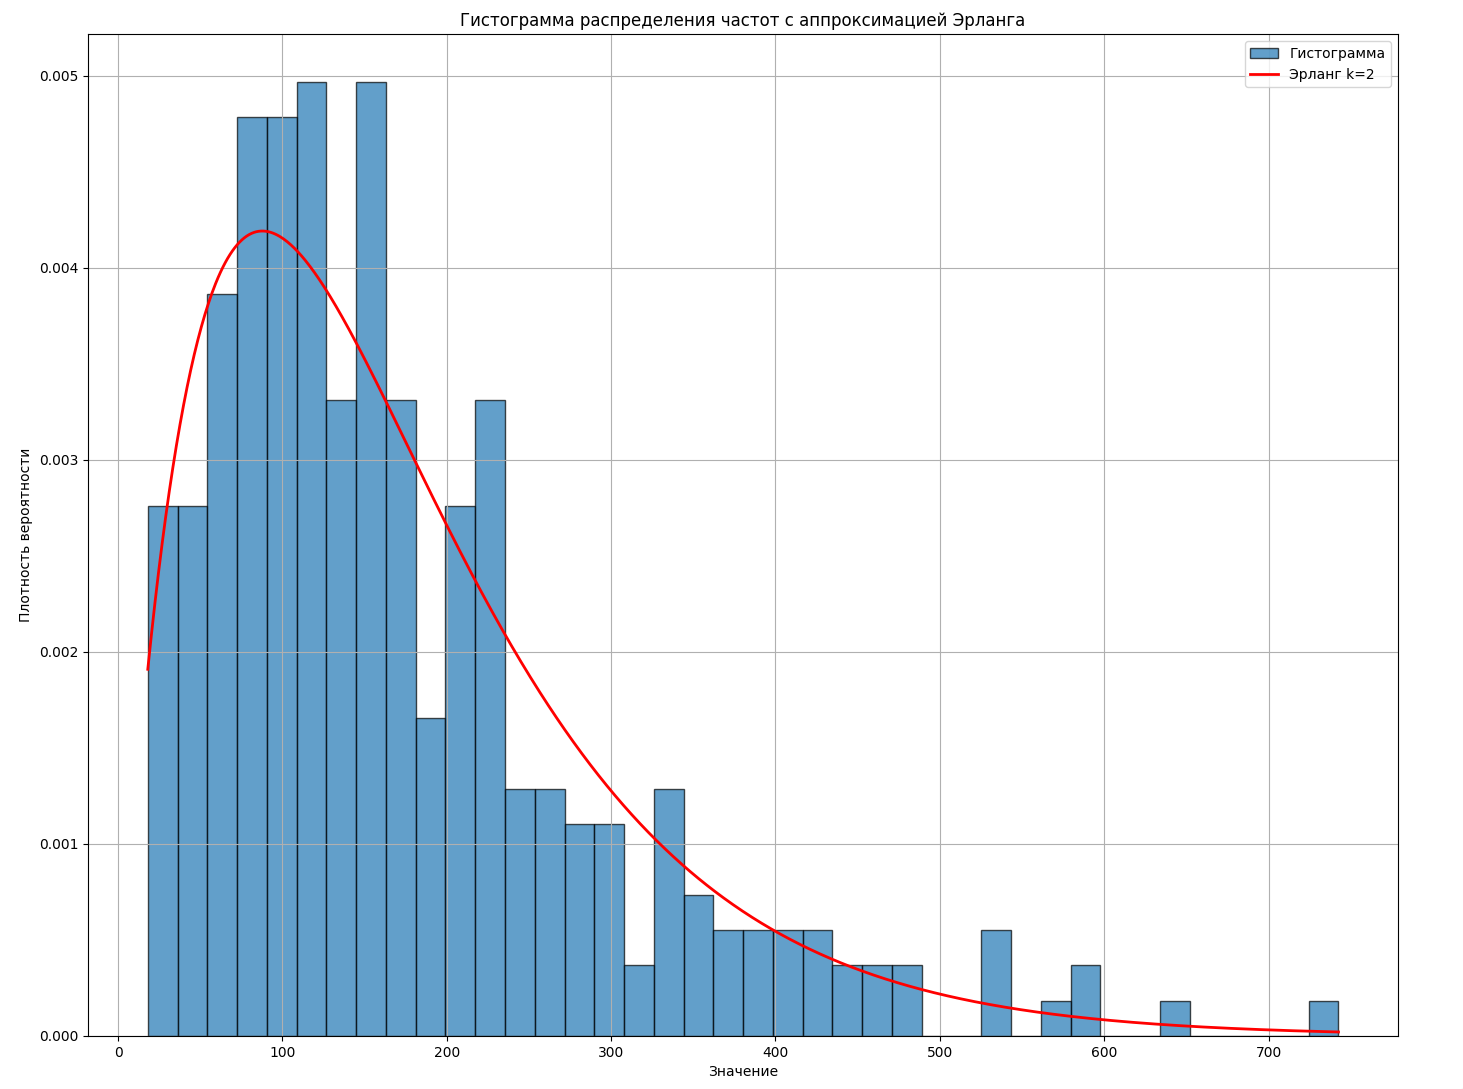
\includegraphics[width=1\textwidth]{../data/histogram_approximated.png}
	\caption{Распределение Эрланга для различных параметров}
\end{figure}
\FloatBarrier

\subsection{Выводы}

Для каждого случая был рассчитан соответствующий параметр \(\lambda\), основанный на среднем значении подвыборок. Аппроксимация показала, что распределение соответствует нормированному закону Эрланга для значений коэффициента вариации.


% -------------------------------

\section{Генерация случайной последовательности}
% \subsection{Программная реализация на языке Python}

Для реализации распределения Эрланга использовался язык программирования Python. Алгоритм заключается в том, что для каждого элемента выборки генерируется сумма \( k \) случайных величин, каждая из которых распределена по экспоненциальному закону с параметром \( \lambda \). Данная сумма соответствует распределению Эрланга с параметрами \( k \) и \( \lambda \).

\begin{lstlisting}
import math
import random

k = 2
lambda_param = 0.0144

def generate_exponential(lambda_param):
    return -math.log(random.random()) / lambda_param

def generate_erlang(k, lambda_param, size=1000):
    erlang_samples = []
    for _ in range(size):
        sample = sum(
            generate_exponential(lambda_param) for _ in range(k)
        )
        erlang_samples.append(sample)
    return erlang_samples

generated_data = generate_erlang(k, lambda_param)
\end{lstlisting}

Генерация данных проводится с помощью функции `generate\_erlang`, которая для каждой случайной величины просуммирует \( k \) экспоненциальных случайных величин, сгенерированных с параметром \( \lambda \).

\subsection{Выводы}

Алгоритм генерации случайных величин по закону Эрланга был успешно реализован, что позволяет получать величины, соответствующие этому распределению, для дальнейшего анализа.


% -------------------------------

\section{Сравнительный анализ}
% \subsection{Аппроксимирующий закон и исходная ЧП}

В ходе выполнения работы было выполнено аппроксимирующее моделирование исходной числовой последовательности с использованием распределения Эрланга с порядком \( k = 2 \).

На рисунке 7 представлена гистограмма для случайных величин, сгенерированных в соответствии с этим законом распределения, а на рисунке 8 — гистограмма распределения частот исходной числовой последовательности.

\begin{figure}[H]
	\centering
	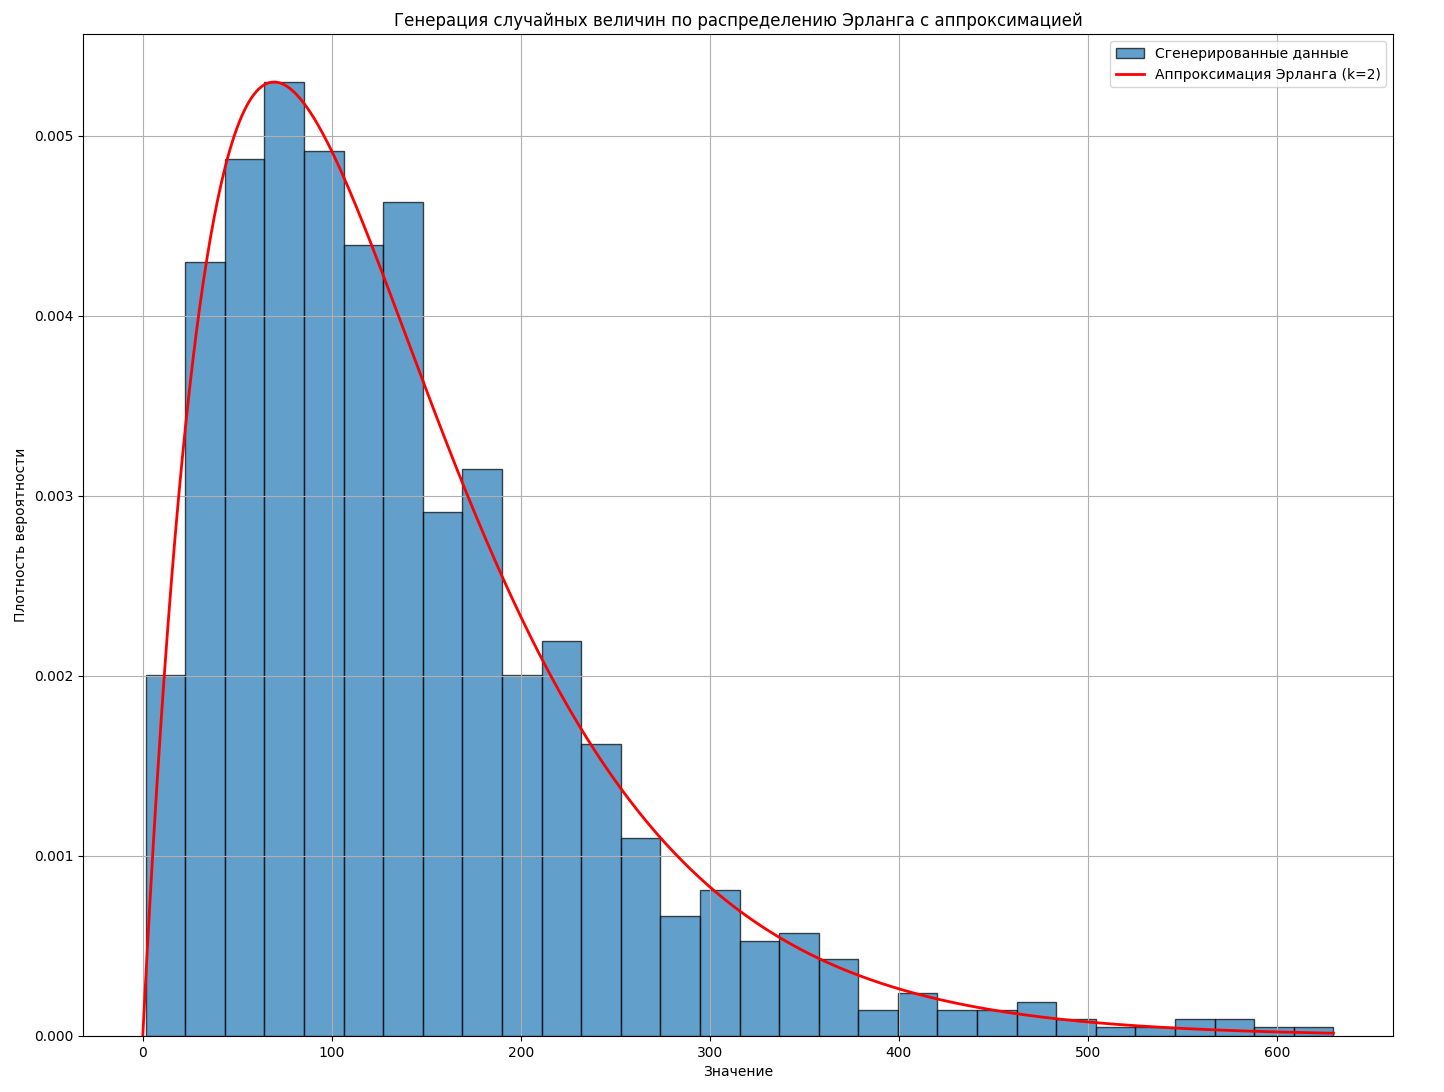
\includegraphics[width=1\textwidth]{../data/histogram_random_generated.png}
	\caption{Распределение Эрланга для сгенерированной последовательности}
\end{figure}

\begin{figure}[H]
	\centering
	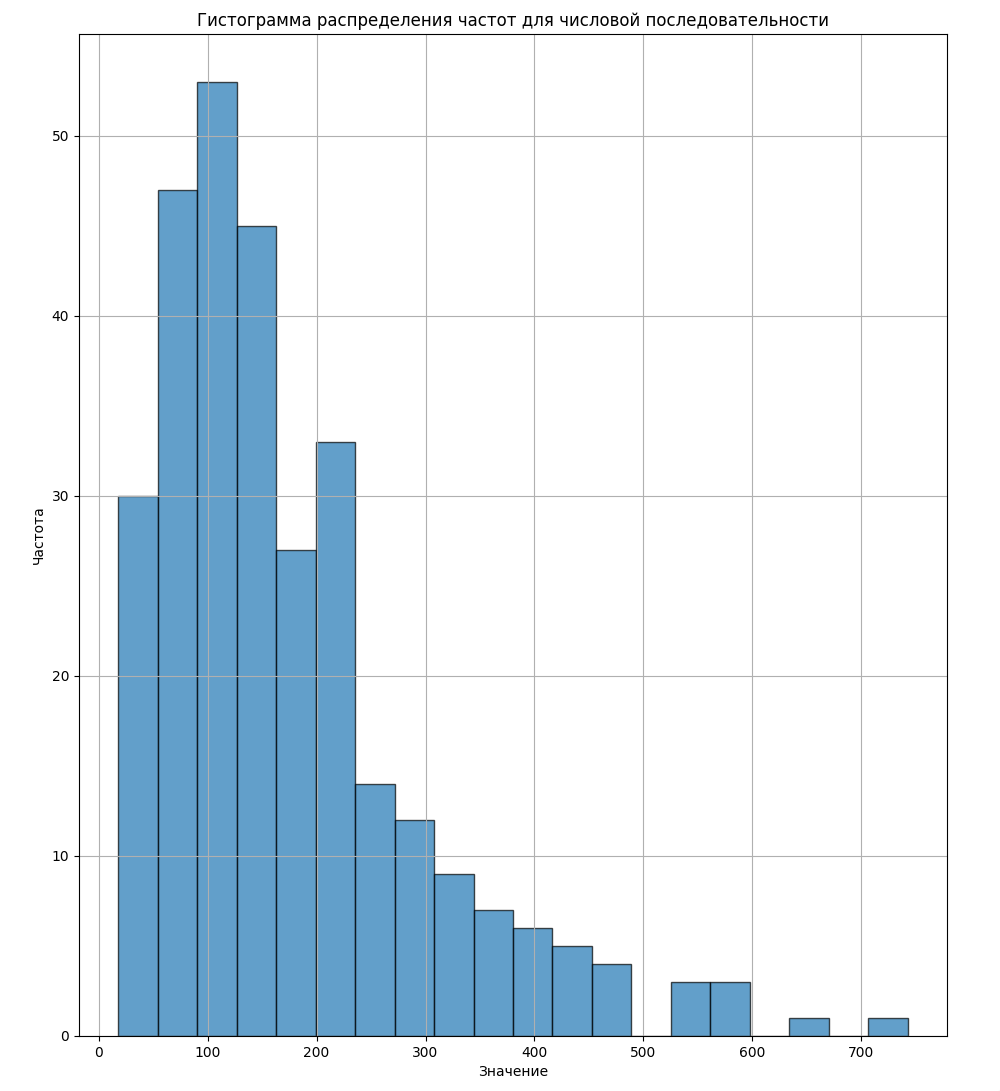
\includegraphics[width=0.8\textwidth]{../data/histogram.png}
	\caption{Гистограмма распределения частот заданной ЧП}
\end{figure}

На основании представленных гистограмм можно сделать вывод, что плотности распределения для сгенерированной по закону Эрланга последовательности и исходной числовой последовательности имеют схожие формы. Гистограммы отображают аналогичное распределение частот, что указывает на правильность выбора аппроксимирующего закона. Несмотря на возможные незначительные отличия в локальных частотах, общая картина подтверждает, что распределение Эрланга хорошо описывает исходную числовую последовательность. Данный результат также подтверждается тем, что коэффициенты вариации и другие числовые характеристики сгенерированных данных находятся в приемлемых пределах отклонений от исходных значений.

\subsection{Форма 2: Таблица числовых моментов для различных выборок}
В таблице ниже представлены числовые моменты для выборок из 10, 20, 50, 100, 200 и 300 значений. Для каждой подвыборки вычислены математическое ожидание, дисперсия, среднеквадратическое отклонение, коэффициент вариации и доверительные интервалы для различных уровней доверия, а также относительные отклонения рассчитанных значений от величин, полученных для выборки из 300 значений.

\FloatBarrier
\begin{table}[H]
	\centering
	\resizebox{\textwidth}{!}{
		\begin{tabular}{|c|c|c|c|c|c|c|c|}
			\hline
			\multirow{2}{*}{\textbf{Характеристика}}   &      & \multicolumn{6}{c|}{\textbf{Количество случайных величин}}                                                                                        \\
			\cline{2-8}
			                                           &      & \textbf{10}                                                & \textbf{20} & \textbf{50} & \textbf{100} & \textbf{200} & \textbf{300}               \\
			\hline
			\multirow{2}{*}{\textbf{Мат. ожидание}}    & Знач & 158.251                                                    & 157.526     & 148.864     & 146.513      & 142.194      & \multirow{2}{*}{141.211}   \\
			\cline{2-7}
			                                           & $\%$ & 12.067\%                                                   & 11.553\%    & 5.420\%     & 3.755\%      & 0.697\%      &                            \\
			\hline
			\multirow{2}{*}{\textbf{Дов. инт. (0.9)}}  & Знач & \pm78.005                                                  & \pm45.096   & \pm24.558   & \pm18.992    & \pm12.609    & \multirow{2}{*}{\pm10.018} \\
			\cline{2-7}
			                                           & $\%$ & 678.670\%                                                  & 350.159\%   & 145.146\%   & 89.579\%     & 25.864\%     &                            \\
			\hline
			\multirow{2}{*}{\textbf{Дов. инт. (0.95)}} & Знач & \pm96.263                                                  & \pm54.586   & \pm29.436   & \pm22.696    & \pm15.046    & \multirow{2}{*}{\pm11.948} \\
			\cline{2-7}
			                                           & $\%$ & 705.661\%                                                  & 356.854\%   & 146.364\%   & 89.948\%     & 25.925\%     &                            \\
			\hline
			\multirow{2}{*}{\textbf{Дов. инт. (0.99)}} & Знач & \pm138.292                                                 & \pm74.613   & \pm39.256   & \pm30.041    & \pm19.844    & \multirow{2}{*}{\pm15.740} \\
			\cline{2-7}
			                                           & $\%$ & 778.624\%                                                  & 374.049\%   & 149.409\%   & 90.862\%     & 26.074\%     &                            \\
			\hline
			\multirow{2}{*}{\textbf{Дисперсия}}        & Знач & 18107.943                                                  & 13603.345   & 10728.201   & 13082.825    & 11643.061    & \multirow{2}{*}{11058.907} \\
			\cline{2-7}
			                                           & $\%$ & 63.741\%                                                   & 23.008\%    & -2.990\%    & 18.301\%     & 5.282\%      &                            \\
			\hline
			\multirow{2}{*}{\textbf{Ср. кв. о.}}       & Знач & 134.566                                                    & 116.633     & 103.577     & 114.380      & 107.903      & \multirow{2}{*}{105.161}   \\
			\cline{2-7}
			                                           & $\%$ & 27.961\%                                                   & 10.909\%    & -1.507\%    & 8.766\%      & 2.607\%      &                            \\
			\hline
			\multirow{2}{*}{\textbf{Коэф. вариации}}   & Знач & 85.033\%                                                   & 74.041\%    & 69.578\%    & 78.068\%     & 75.884\%     & \multirow{2}{*}{74.471\%}  \\
			\cline{2-7}
			                                           & $\%$ & 14.183\%                                                   & -0.578\%    & -6.570\%    & 4.830\%      & 1.897\%      &                            \\
			\hline
		\end{tabular}}
	\caption{Числовые моменты для различных выборок ЧП}
\end{table}
\FloatBarrier


\subsection{Результаты автокорреляционного анализа}

Для оценки случайности последовательности использовалось пороговое значение коэффициента автокорреляции — 0.2. Если автокорреляция на сдвиге превышает это значение, последовательность можно считать неслучайной. Но как видно из талицы и графика, ни одно из значений коэффициентов корелляции для исходной последовательности не превышает даже 0,1 -- исходя из этого можно сделать вывод, что числовая последовательность является случайной.

\begin{table}[H]
	\centering
	\resizebox{\textwidth}{!}{
		\begin{tabular}{|c|c|c|c|c|c|c|c|c|c|c|}
			\hline
			\textbf{Сдвиг ЧП}                     & \textbf{1} & \textbf{2} & \textbf{3} & \textbf{4} & \textbf{5} & \textbf{6} & \textbf{7} & \textbf{8} & \textbf{9} & \textbf{10} \\
			\hline
			\textbf{К-т АК} для сген. \textbf{ЧП} & 0.0185     & 0.0372     & 0.0238     & -0.0298    & 0.0550     & 0.0055     & -0.0226    & 0.0331     & -0.0164    & -0.0055     \\
			\hline
		\end{tabular}
	}
	\caption{Коэф. автокорреляции для сгенерированной ЧП}
\end{table}


\begin{figure}[H]
	\centering
	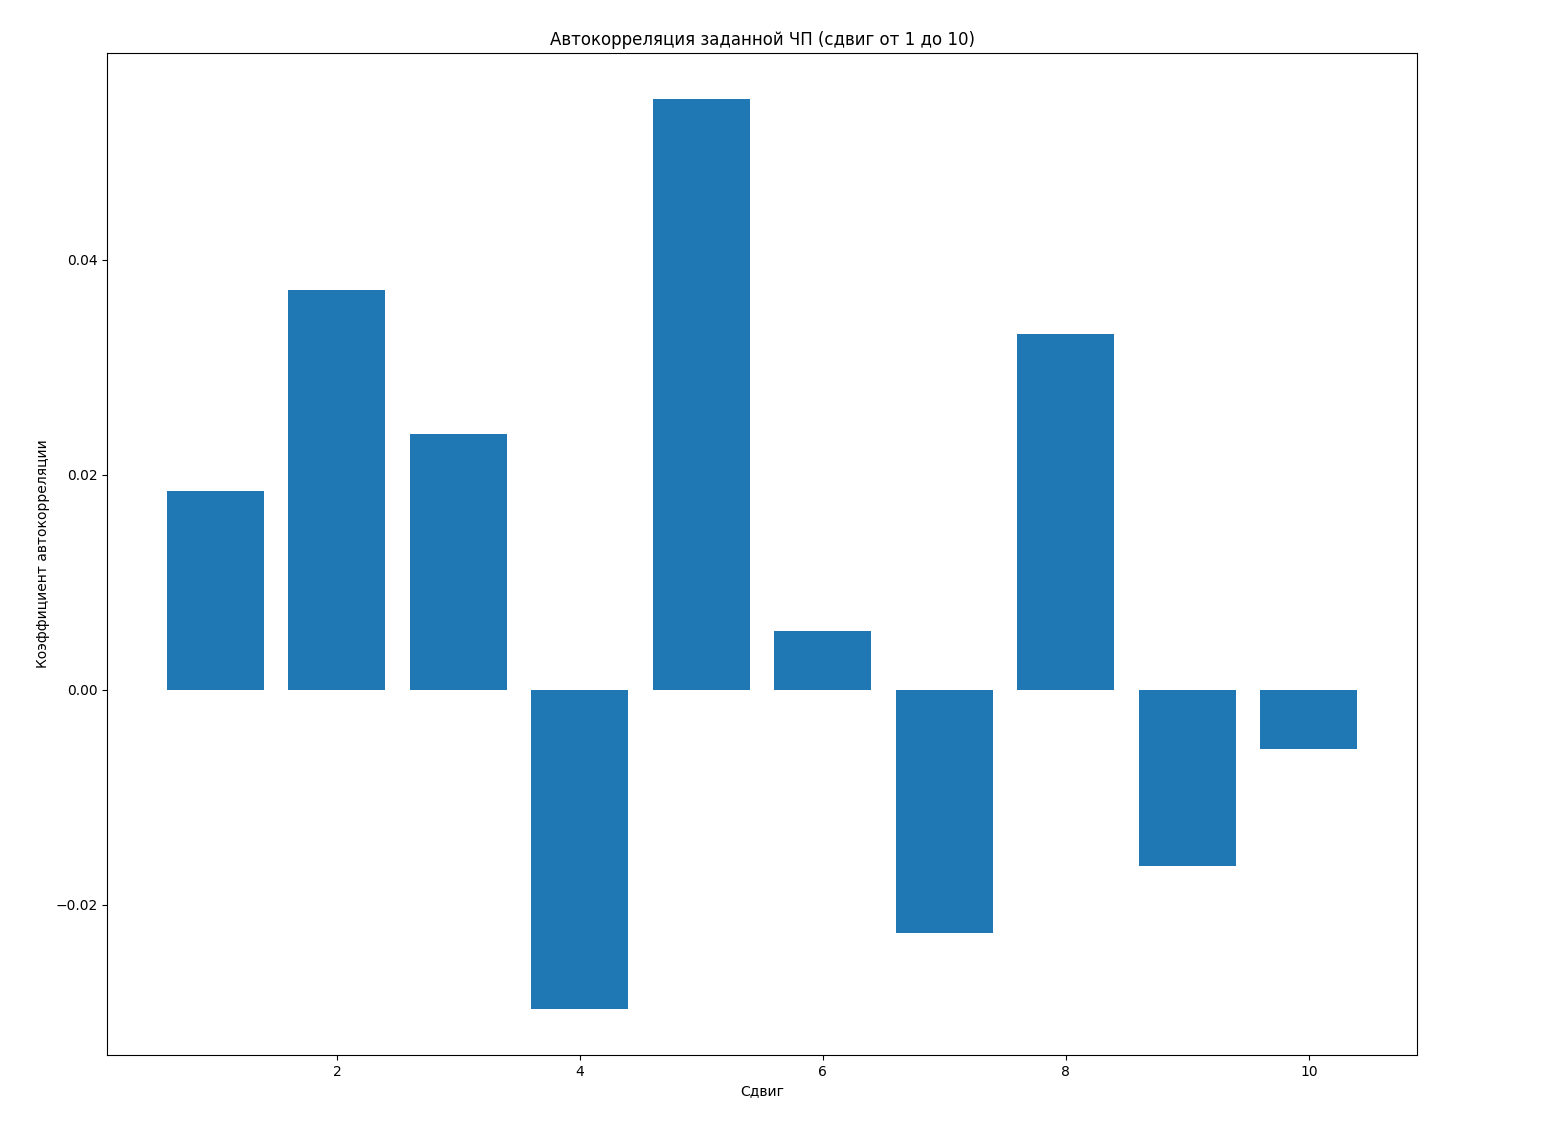
\includegraphics[width=1\textwidth]{../data/auto_corellation_random-2.png}
	\caption{Автокорреляционный анализ для сгенерированной(заданной в этом пункте) числовой последовательности}
\end{figure}

\subsection{Выводы}

\begin{itemize}
	\item В результате проведенного анализа аппроксимации исходной числовой последовательности было установлено, что распределение Эрланга с порядком \( k = 2 \) является подходящим законом распределения для моделирования заданной числовой последовательности. Это подтверждается визуальным сходством гистограммы распределения частот для исходной последовательности и сгенерированной последовательности на основе аппроксимирующего закона.

	\item Расчет числовых характеристик для сгенерированной последовательности, таких как математическое ожидание, дисперсия, среднеквадратическое отклонение и коэффициент вариации, показал, что значения сгенерированных данных находятся в пределах допустимых отклонений от исходных значений. Средние значения и другие статистические моменты подтвердили точность аппроксимации закона распределения.

	\item Автокорреляционный анализ для сгенерированной последовательности показал, что значения коэффициентов автокорреляции не превышают критического порога (0.2), что свидетельствует о случайности последовательности. Этот результат сопоставим с автокорреляционным анализом исходной числовой последовательности, подтверждая, что случайная природа последовательности сохраняется после моделирования.

	\item В целом, выполненные шаги по аппроксимации и сравнению исходной числовой последовательности с сгенерированной в соответствии с законом распределения Эрланга показали высокую степень соответствия, как по визуальным, так и по числовым характеристикам. Таким образом, выбор данного закона для аппроксимации оказался обоснованным и эффективным.
\end{itemize}


% -------------------------------

\section{Выводы по работе}

Вывод по работе

\end{document}
